\documentclass{article}

\usepackage{amsmath}
\usepackage{tikz}
\usepackage{graphicx}

\title{Turing Machine Documentation}
\author{Ryan Peruski, Maria Hernandez}
\date{\today}

\begin{document}

\maketitle
\section{Roles}

\begin{itemize}
    \item Ryan Peruski: Created initial stack design and initial templates for the documentation. Revised the machine and suggested improvements. Added examples to the documentation.
    \item Maria Hernandez: Edited the stack design to adapt to the specific problem of "valid parentheses", added string and character constant parsing sections, and multi-line comments section
    in the TM and the documentation. Added examples in the documentation.
\end{itemize}

\section{Definition}
This Turing Machine can input any C-code and it places opening parentheses, square brackets, curly brackest, or opening,
multi-line comment on the stack and pop their respective closing operators. If the machine encounters a closing operator and 
it does not see the matching operator of the right type on the top of the stak (represented by the first blank to the right), 
it rejects. If the Turing Machine finishes reading the input and there is something on the stack, it will reject. 
If the original input is empty, it will accept. 

In addition, this Turning Machine pseudo-parses strings and constant characters, by applying certain syntax rules explained below. 

\section{States, Transitions, Image}
The Turing machine operates by moving between states and performing transitions on the tape. The states and transitions are labeled as follows:

\begin{itemize}
    \item $Red$ Reject states ($q_{reject}$)
    \item $Green$ Accept state ($q_{accept}$)
    \item $Blue$ Single quotes parsing
    \item $Pink$ Double quotes parsing
    \item $Cyan$ Stack's push states  
    \item $Light Coral$ Stack's pop states
    \item $Purple$ Multi-line comments section 
    \item $Black$ Initial states to set up the $\#$
    \item $Beige$ Transition state (between stack push operations, pop operations, single quotes and double quotes parsing, and multi-line comments)
    \item $Gray$ State to determine the validity of the original input tape
\end{itemize}

Finally, the Turing Machine is shown in Figure\ \ref{fig:stackqueue}.
\begin{figure}
    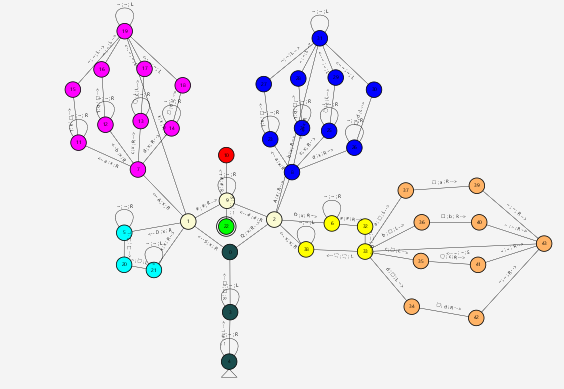
\includegraphics[width=\linewidth]{stackqueue.png}
    \caption{Turing Machine.}\label{fig:stackqueue}
\end{figure}


\section{Machine Specifications}

\begin{itemize}
    \item Input Alphabet: Any ASCII symbol, except #, x, and space
    \item Tape Alphabet:  Any ASCII symbol, including #, x, and space
\end{itemize}

\subsection{Characters reserved for the tape alphabet}
The following are reserved characters: #, x, and spaces. Meaning that they are part of the tape alphabet, but cannot be part of the 
input alphabet. # is reserved to delimit the end of the original input tape, as soon as the machine starts running it will mark the 
end of the original input data. X is reserved to mark the characters that have been already read from the original input data. 
Space is reserved to know the following: 1. where to place the #, 2. where to start reading the original input data (after placing 
the # and going back), 3. whether the stack is empty or not after finishing reading the original input tape.

The tape will be divided by a #. Anything before the # represents the original input data (code), and everything after the 
# represents the stack. 

\subsection{How to start the machine}
In the original tape, enter any character belonging to the input alphabet (do not enter #, x, or space, or the machine will not work properly). 
The start state is the state 0. The first thing the machine will do when the machine starts running is to place the # to delimit the end of the 
original input data (usually C-code) and the beginning of the "stack". The only elements that can be placed on the stack are the opening 
operators - namely, (,{,[,/* 

\section{Functional Description of the Turing Machine}

\subsection{Valid (,),[,],{,} - exception}
As previously mentioned, the TM evaluates whether the (,{,[ characters in the original input data have their corresponding closing ],},). 
There is an exception when these characters are either inside double quotes or multi-line comments /**/. For instance, the machine will 
accept /*{*/ and ")" since in C anything inside /**/ is ignored and, C allows us to write anything inside "".

\subsection{Double quote section ""}
This TM is not evaluating the parity of "", but also other syntax properties of C. If the original input data contains double quotes, 
the only way the machine will accept it is if it has an even number of double quotes. Namely, it accepts if after opening a double quote, and writing 
any character in the string, the TM finds the respective closing double quote – the only way to ensure that in the machine is if we go back to state 2. 
There is an exception to this rule, the TM may accept an uneven number of " only if some of them are preceded by a \ (escape character). 
After the escape character \ only certain characters are allowed (",n,0,',a,b,f,r,t,v,\,?), we did not account for escape sequences for octal 
numbers \000 and hexadecimal numbers \xhh since that would have made the TM needlessly complicated.

If the TM is curretly at state 28 and it reads a # the original input data has an uneven number of ", hence the machine rejects the string (ex: "Hello""). 
If the TM reads a escape character \ in state 28, it goes to state 29. If the TM is at state 29 and the following character in the tape is not any of 
the special sequence characters or if there are not more characters from the initial data (next character is #), then the machine rejects the string 
(ex: "\k, "\). State 30 allows the TM to either read a new escape character (\), go back to state 2 - if reading a closing ", read any other element 
on the string, or reject the string if reading a #. 

\subsection{Single quote section}

This TM is not evaluating the parity of '', but also other syntax properties of C, including, not accepting empty character '' or accepting certain escape 
sequence characters (the same ones double quotes accept). The only way to accept an input containing single quotes is if it contains an opening and closing '. 
An uneven number of ' may be accepted if ' is preceded by a escape character \. Even though the usage of multicharacter constants is not strictly prohibited in C,
functions like putc are designed to output only a single character. Hence, when including multicharacters in '', putc, for instance, will likely just output the 
lowest byte of the integer – if the machine is little endian. Due to this behavior we are restricting our machine to only accept one character (maximum two if the 
input tape includes the escape sequence) between ''. If while in state 31, the machine reads a # (end of original input tape), or a ', the machine rejects because 
either there is an opening' without its corresponding closing ', or because it is an empty character. If while in state 32, the machine reads another character 
other than the closing ', the machine rejects the input – this machine does not allow multiple characters inside ''. 

\subsection{Comments}

The operators that gave us the most work were /* and */. Since the tape reads one character at a time, we needed to take into account several possible scenarios 
so that the machine always halt, and correctly behaves in cases when the original tape has something like *{/}, or /(*), or, *(*), or *[/} (reject in this case). 
Reason why there are a lot of transitions coming out of states 24 and 25. Also, we needed a special branch (purple branch) for the comments so that we could 
ignore everything inside /* */.

As with [, (, and { if the TM reads a / followed by a *, it X them out, and them place them on the “stack” section. Then the machine goes back and X out all characters 
until reading both a * followed by a /. The machine rejects if while reading characters, it finds the end of the original input tape # before finding */ 
(ex: state of TM after placing #: /*Hello#, /*Hello*#, /*Hello***#). If the TM reads a */ in the original input tape, and it does not find the corresponding opening 
/* in the stack section, it rejects (ex: */#, Hello*/#). If the TM finds nested comments, it rejects (ex: /*/**/*/#, /*/*****H**i*/*/), in this case the /* inside /**/ 
is considered a comment, thus is ignored, onsequently the last */ will not have its corresponding opening /*. Everything inside the comments is ignored, hence in this 
case the TM allows single {,[,(,),],}. 

Since, to be able to correctly implement the comments this machine needs to find two consecutives characters in the input tape. The TM accounts for cases when it reads
from the input tape a * or / immediately followed by one of the other special characters  {,[,(,),],},”,’,#, this is why states 24 and 25 have several transitions. 

\section{Examples}
Here are some examples of input and output for the Turing machine:
\begin{itemize}
    \item \begin{verbatim} Input: v[i]=a[i][j];, Output:  xxxxxxxxxxxxx#, ACCEPTS \end{verbatim}
    \item \begin{verbatim} Input: for(;;)break;, Output:   xxxxxxxxxxxxx#, ACCEPTS \end{verbatim}
    \item \begin{verbatim} Input: {x=7}, Output:  xxxxx#, ACCEPTS \end{verbatim}
    \item \begin{verbatim} Input: for(i=0;i<v.size();i++)v[i]=2;, Output: xxxxxxxxxxxxxxxxxxxxxxxxxxxxxx#, ACCEPTS \end{verbatim}
    \item \begin{verbatim} Input: v[i]=a[i, Output:  xxxxxxxx#[, REJECTS \end{verbatim}
    \item \begin{verbatim} Input: for(;;, Output: xxxxxx#(, REJECTS \end{verbatim}
    \item \begin{verbatim} Input: printf("HelloWorld!\n");, Output: xxxxxxxxxxxxxxxxxxxxxxxx#, ACCEPTS \end{verbatim}
    \item \begin{verbatim} Input: printf("Hereisa{(");, Output:  xxxxxxxxxxxxxxxxxxxx#, ACCEPTS \end{verbatim}
    \item \begin{verbatim} Input: """, Output: xxx#, REJECTS \end{verbatim}
    \item \begin{verbatim} Input: 'a''\n', Output:  xxxxxxx#, ACCEPTS \end{verbatim}
    \item \begin{verbatim} Input: /*WeSupportComments!*/, Output: xxxxxxxxxxxxxxxxxxxxxx#, ACCEPTS \end{verbatim}
    \item \begin{verbatim} Input: /*WeSupportComments!{{{{*/, Output: xxxxxxxxxxxxxxxxxxxxxxxxxx#, ACCEPTS \end{verbatim}
    \item \begin{verbatim} Input: /*/*/, Output: xxxxx# , ACCEPTS \end{verbatim}  
    \item \begin{verbatim} Input: /*/*, Output: xxxx#/* , REJECTS \end{verbatim}
    \item \begin{verbatim} Input: */*/, Output:  xx*/#  , REJECTS \end{verbatim}
    \item \begin{verbatim} Input: /*a*b*/, Output: xxxxxxx# , ACCEPTS \end{verbatim}
    \item \begin{verbatim} Input: /*HelloWorld*/*/, Output: xxxxxxxxxxxxxxxx#  , REJECTS \end{verbatim}
    \item \begin{verbatim} Input: /*/**/, Output:  xxxxxx# , ACCEPTS, NOTE: It accepts because it treats the inner /* as comment, but normal compilers throw a warning in these cases \end{verbatim} 
    \item \begin{verbatim} Input: /*}*/, Output: xxxxx# , ACCEPTS, NOTE: } doesn't have the opening {, but this accepts because it treats anything inside /**/ as comments \end{verbatim}
    \item \begin{verbatim} Input: /*/**/*/, Output: xxxxxxxx# , REJECTS, NOTE: last */ does not have an opening /*. Compilers do not accept nested comments \end{verbatim}
    \item \begin{verbatim} Input: /*a*b* , Output: xxxxxx#/*  , REJECTS \end{verbatim}
    \item \begin{verbatim} Input: (/, Output:  xx#( , REJECTS \end{verbatim} 
    \item \begin{verbatim} Input: (/*****)*/* , Output:  xxxxxxxxxxx#( , REJECTS, NOTE: needs closing ) \end{verbatim}
    \item \begin{verbatim} Input: (/*****)*/*), Output:  xxxxxxxxxxxx# , ACCEPTS \end{verbatim}
    \item \begin{verbatim} Input: (/*****)*/*)*, Output:  xxxxxxxxxxxxx# , ACCEPTS \end{verbatim}
    \item \begin{verbatim} Input: (/*)Hi***/}"", Output: xxxxxxxxxxx""#( , REJECTS, Note: rejects as soon as } doenst match ( \end{verbatim}
    \item \begin{verbatim} Input: *{/}, Output:  xxxx# , ACCEPTS \end{verbatim}
    \item \begin{verbatim} Input: /(*), Output:  xxxx# , ACCEPTS \end{verbatim}
    \item \begin{verbatim} Input: *(*), Output:  xxxx# , ACCEPTS \end{verbatim}
    \item \begin{verbatim} Input: *[/}, Output:  xxxx# , ACCEPTS \end{verbatim}
    \item \begin{verbatim} Input: '\k', Output:   xxx'# , REJECTS \end{verbatim}
    \item \begin{verbatim} Input: '\n, Output:   xxx# , REJECTS \end{verbatim}
    \item \begin{verbatim} Input: 'a', Output:  xxx# , ACCEPTS \end{verbatim}
    \item \begin{verbatim} Input: '\'', Output:  xxxx# , ACCEPTS \end{verbatim}
    \item \begin{verbatim} Input: "\"\0"\'\r", Output: xxxxxxxxxxx# , REJECTS \end{verbatim}
    \item \begin{verbatim} Input: "\"\0"\'\r', Output:  xxxxxxxxxxx# , ACCEPTS - The TM is evaluating the parity of "" and '' (it is not evaluating 
        whether it makes sense for C to divide "\"\0" by '\r' \end{verbatim} 
    \item \begin{verbatim} Input: "\tHello\\\", Output: xxxxxxxxxxxx# , REJECTS \end{verbatim}
    \item \begin{verbatim} Input: "\tHello\\\"", Output:  xxxxxxxxxxxxx# , ACCEPTS \end{verbatim}
    \item \begin{verbatim} Input: /"\tHi", Output:  xxxxxxx# , ACCEPTS \end{verbatim}
    \item \begin{verbatim} Input: "{"{[/*}*/]}, Output:  xxxxxxxxxxxx# , ACCEPTS \end{verbatim}
    \item \begin{verbatim} Input: '{'{[/*/*(}[*/]}, Output:  xxxxxxxxxxxxxxxx# , ACCEPTS \end{verbatim} 
    \item \begin{verbatim} Input: "{"{[/*/**/]}, Output:  xxxxxxxxxxxxx# , ACCEPTS \end{verbatim}
    \item \begin{verbatim} Input: "{"{(/*/*(}[*/]}, Output:   xxxxxxxxxxxxxxx}#{( , REJECTS \end{verbatim}

\end{itemize}

\section{Conclusion}
This Turing Machine represents a system designed specifically for processing and analyzing C code. Its primary function is to systematically evaluate 
the syntactical correctness of parentheses, brackets, and comment structures within C code, ensuring that each opening symbol has a corresponding and 
appropriately placed closing symbol. The machine achieves this by utilizing a state transition mechanism that accounts for various scenarios and 
exceptions inherent in C syntax.

Key Features:

\begin{itemize}
\item \begin{verbatim} Handling of Code Structures: The TM adeptly manages typical C code constructs, including parentheses, square brackets, and curly brackets, ensuring that 
they are correctly paired and nested. This includes special handling for code within double quotes, single quotes, and comments, where the usual syntax rules differ. \end{verbatim}
\item \begin{verbatim} Complex State Transitions: The machine is equipped with a range of states to handle different aspects of C code syntax. These states enable pseudo-parse string 
literals and constant characters and dealing with comment blocks. \end{verbatim}
\item \begin{verbatim} Reserved Characters: The use of reserved characters (#, x, and spaces) is a critical aspect of the TM's design. These characters facilitate the machine's operations, 
such as marking the end of input data and tracking read characters, without interfering with the input code analysis. \end{verbatim}
\item \begin{verbatim} Syntax Rule Application: The machine pseudo-parses strings and characters by applying specific syntax rules of C. This includes handling escape sequences within 
strings and ensuring the correct use of single and double quotes. \end{verbatim}
\item \begin{verbatim} Error Detection and Rejection Criteria: The TM is designed to reject incorrect code structures, such as unmatched parentheses or nested comments. \end{verbatim}
\item \begin{verbatim} Special Handling of Comments: This TM ignores content within comment blocks while ensuring the structural integrity of these blocks. \end{verbatim}
\end{itemize}

In summary, this Turing Machine is a specialized and efficient tool for verifying some syntax rules of C code. 

\end{document}